\documentclass[a4paper,12pt]{article}
\usepackage{blindtext}
\usepackage[utf8]{inputenc}
\usepackage[russian]{babel}
\usepackage{graphicx}
\usepackage[left=2cm,right=2cm,top=2cm,bottom=2cm,bindingoffset=0cm]{geometry}
\usepackage{verbatim}
\usepackage{textcomp}
\usepackage{xcolor}
\usepackage{hyperref}
\definecolor{urlcolor}{HTML}{799B03}
\definecolor{linkcolor}{HTML}{799B03}
\hypersetup{pdfstartview=FitH,  linkcolor=linkcolor, urlcolor=urlcolor, colorlinks=true}
\title{JupyterHub x Nbgrader.}
\author{Факультет физики НИУ ВШЭ}
\begin{document}
\maketitle
\tableofcontents
\section{Авторизация} 
Сервер доступен по адресу \url{51.68.81.44/}

 При первой авторизации, если Вам не дали пароль, можно ввести любую комбинацию. JupyterHub запомнит этот пароль, впоследствии изменить его будет очень сложно, пожалуйста, будьте внимательны.

После авторизации вы увидете свою директорию(вкладка files). В ней хранятся скачанные задания. Вы можете изменять содержимое файлов, но не структуру. Названия файлов также не надо менять. Не создавайте дополнительные файлы -- они проверяться не будут, так как сбор домашних заданий автоматизирован.

\begin{figure}[h]
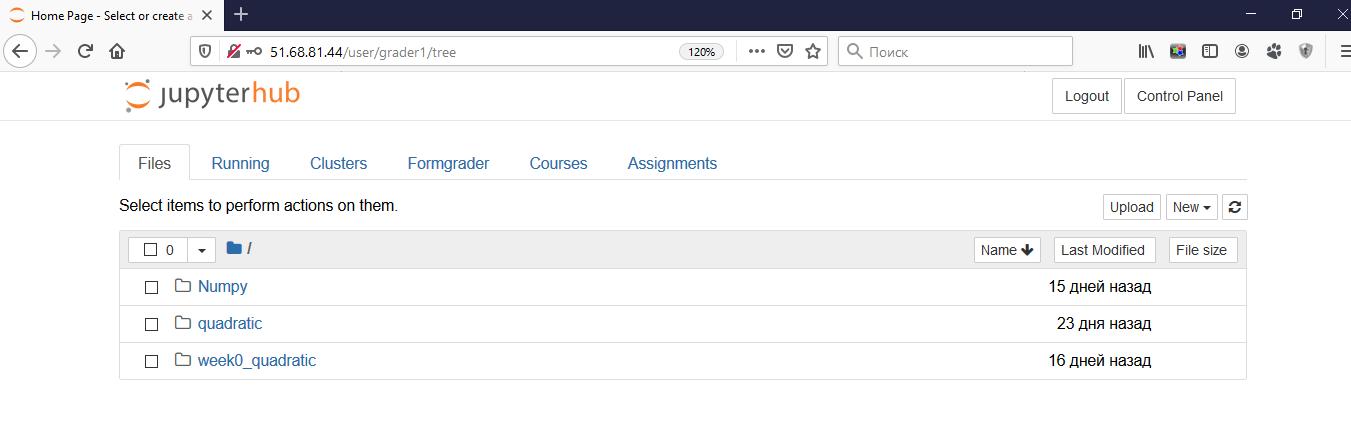
\includegraphics[width=\textwidth]{files}
\end{figure}

Во вкладке Running отображаются все запущенные терминалы и ноутбуки.

\section{Как получить задание}

Все выложенные задания отображаются в вкладке Assignments, в списке Released assignments. Если хотите начать выполнять задание, нажмите кнопку Fetch в строке с соответствующим заданием. Папка с заданием появится в домашней директории (вкладка Files).

\begin{figure}[h]
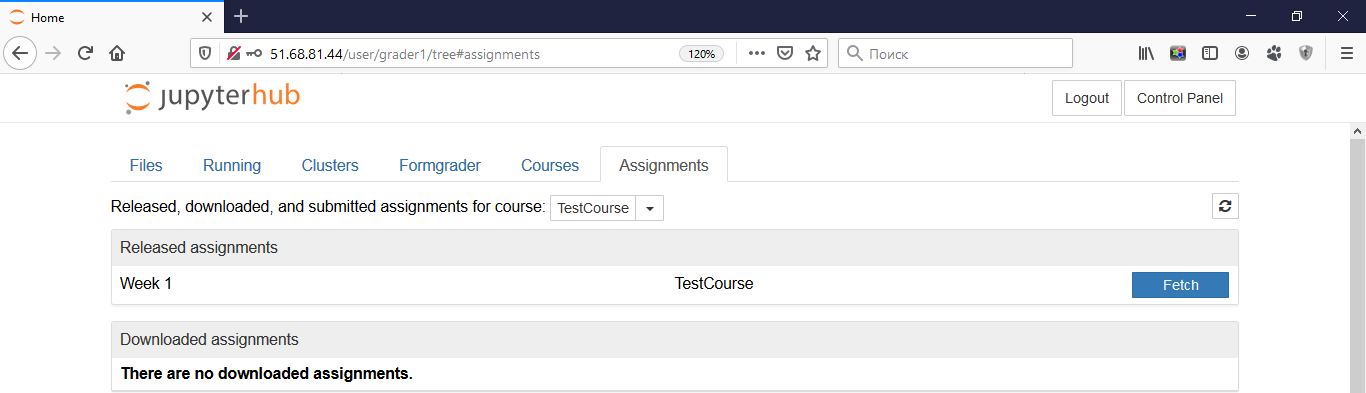
\includegraphics[width=\textwidth]{fetch}
\end{figure}

Также скачанные задания будут отобрачаться в списке Downloaded assignments.

\begin{figure}[h]
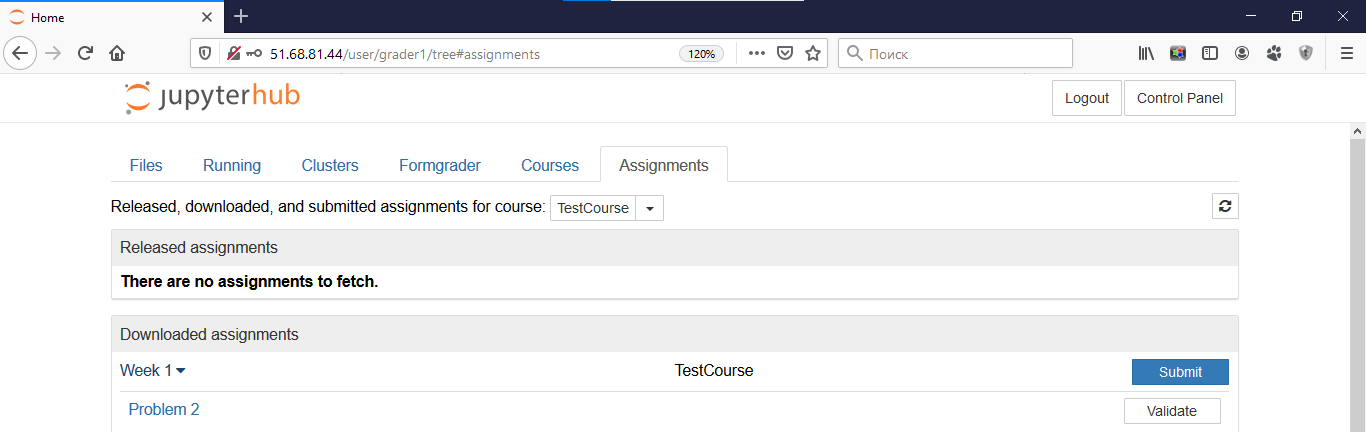
\includegraphics[width=\textwidth]{fetched}
\end{figure}

\section{Как выполнить задание}
В домашней директории откройте файл с заданием. В первой ячейке введите свои данные. Выполняйте задания только в предназначенных для этого ячейках. Если нужно дописать функцию -- не меняйте порядок, имена и количество входных параметров, или имя функции. Это нарушит процесс проверки и задание проверено не будет. Если в задании есть тесты -- проверьте, проходит ли их код запустив соответствующие ячейки, либо кнопкой Validate. Кроме открытых тестов каждое задание содержит скрытые тесты, поэтому проверьте, что код работает не только для открытых тестов. 

В данный момент сервер работает в тестовом режиме и не поддерживает большого количества одновременных запросов и запущенных ядер. Поэтому рекомендуется скачивать файлы с заданиями, выполнять локально и закачивать их назад с помощью кнопки Upload (вкладка files). Также, большая просьба заливать задания не совсем в последний момент: если возникнут неполадаки с сервером, дедлайн будет просрочен. 

Для тех, кто любит рисковать: можно выполнять домашние задания прямо с сервера. Но сохраняйтесь почаще. Если сервер перегрузится, вы увидите кнопку Launch Server либо Start My Server. Нажмите на нее и можете продолжать работать. 

\section{Как отправить выполненное задание}

В вкладке Assignments: downloaded assignments рядом с каждым заданием есть кнопка submit. Нажав на нее, вы отправляете ТЕКУЩУЮ версию своего задания. Если до дедлайна вы отправили задание, а потом изменили его -- можно нажать submit снова, сколько угодно раз. Проверяться будет самая последняя версия, отправленная до дедлайна. 

Перед отправкой задания можно убедиться, что ноутбук проходит все открытые тесты: стрелка рядом с именем задания открывает список ноутбуков этого задания. Каждый из них можно проверить кнопкой validate. Можно отправить задание, не походящее все тесты.

\section{Как узнать свою оценку}

После того как преподаватель проверит задание, в строке submitted assignments появится фунция Fetch feedback. Нажав на нее вы скачаете лист с оценками, разбалловкой и комментариями в домашнюю директорию.
\end{document}